	The limitations for all grammar-based \gls{xml} language solutions reviewed (see Section \ref{sec:literature:schemaLanguages}) require the use of programming languages to validate semantics for questionnaire specifications. These restrictions have led us to design and implement a new authoring language that is non-proprietary, platform independent and use standard formalisms to define structure, data-types, integrity constraints and business rules. This language, uses the state-transition model for routing logic (see Section \ref{sec:cawiLanguage:stateTransition}) together with \gls{rpn} notation to define expressions either for routing or personalisation constructs (see Section \ref{sec:cawiLanguage:rpn}).  

	\gls{cawiml} uses \gls{xsd} to define structure and data types together with \gls{sch} to express integrity constraints and business rules. We have chosen \gls{xsd} due to its well-defined patterns to express vocabulary and structures, its rich set of data-types, its use of \gls{xml} to define constraints and because it is the recommendation schema formalism proposed by \gls{w3c} (see Section \ref{sec:background:xsd}). \gls{sch} adheres to standard \gls{iso}/\gls{iec} 19757 and is also the only rule-based schema language known to address the semantics limitations that grammar-based languages have through XPath query language (see Section \ref{sec:background:sch}). Therefore, to ensure the correctness of \gls{xml} questionnaire instances, we employ a two step process to integrate four different levels of validation. Figure \ref{fig:design:xmlValidation} describes how this process is carried out.

	\begin{figure}[h]
	\centering
	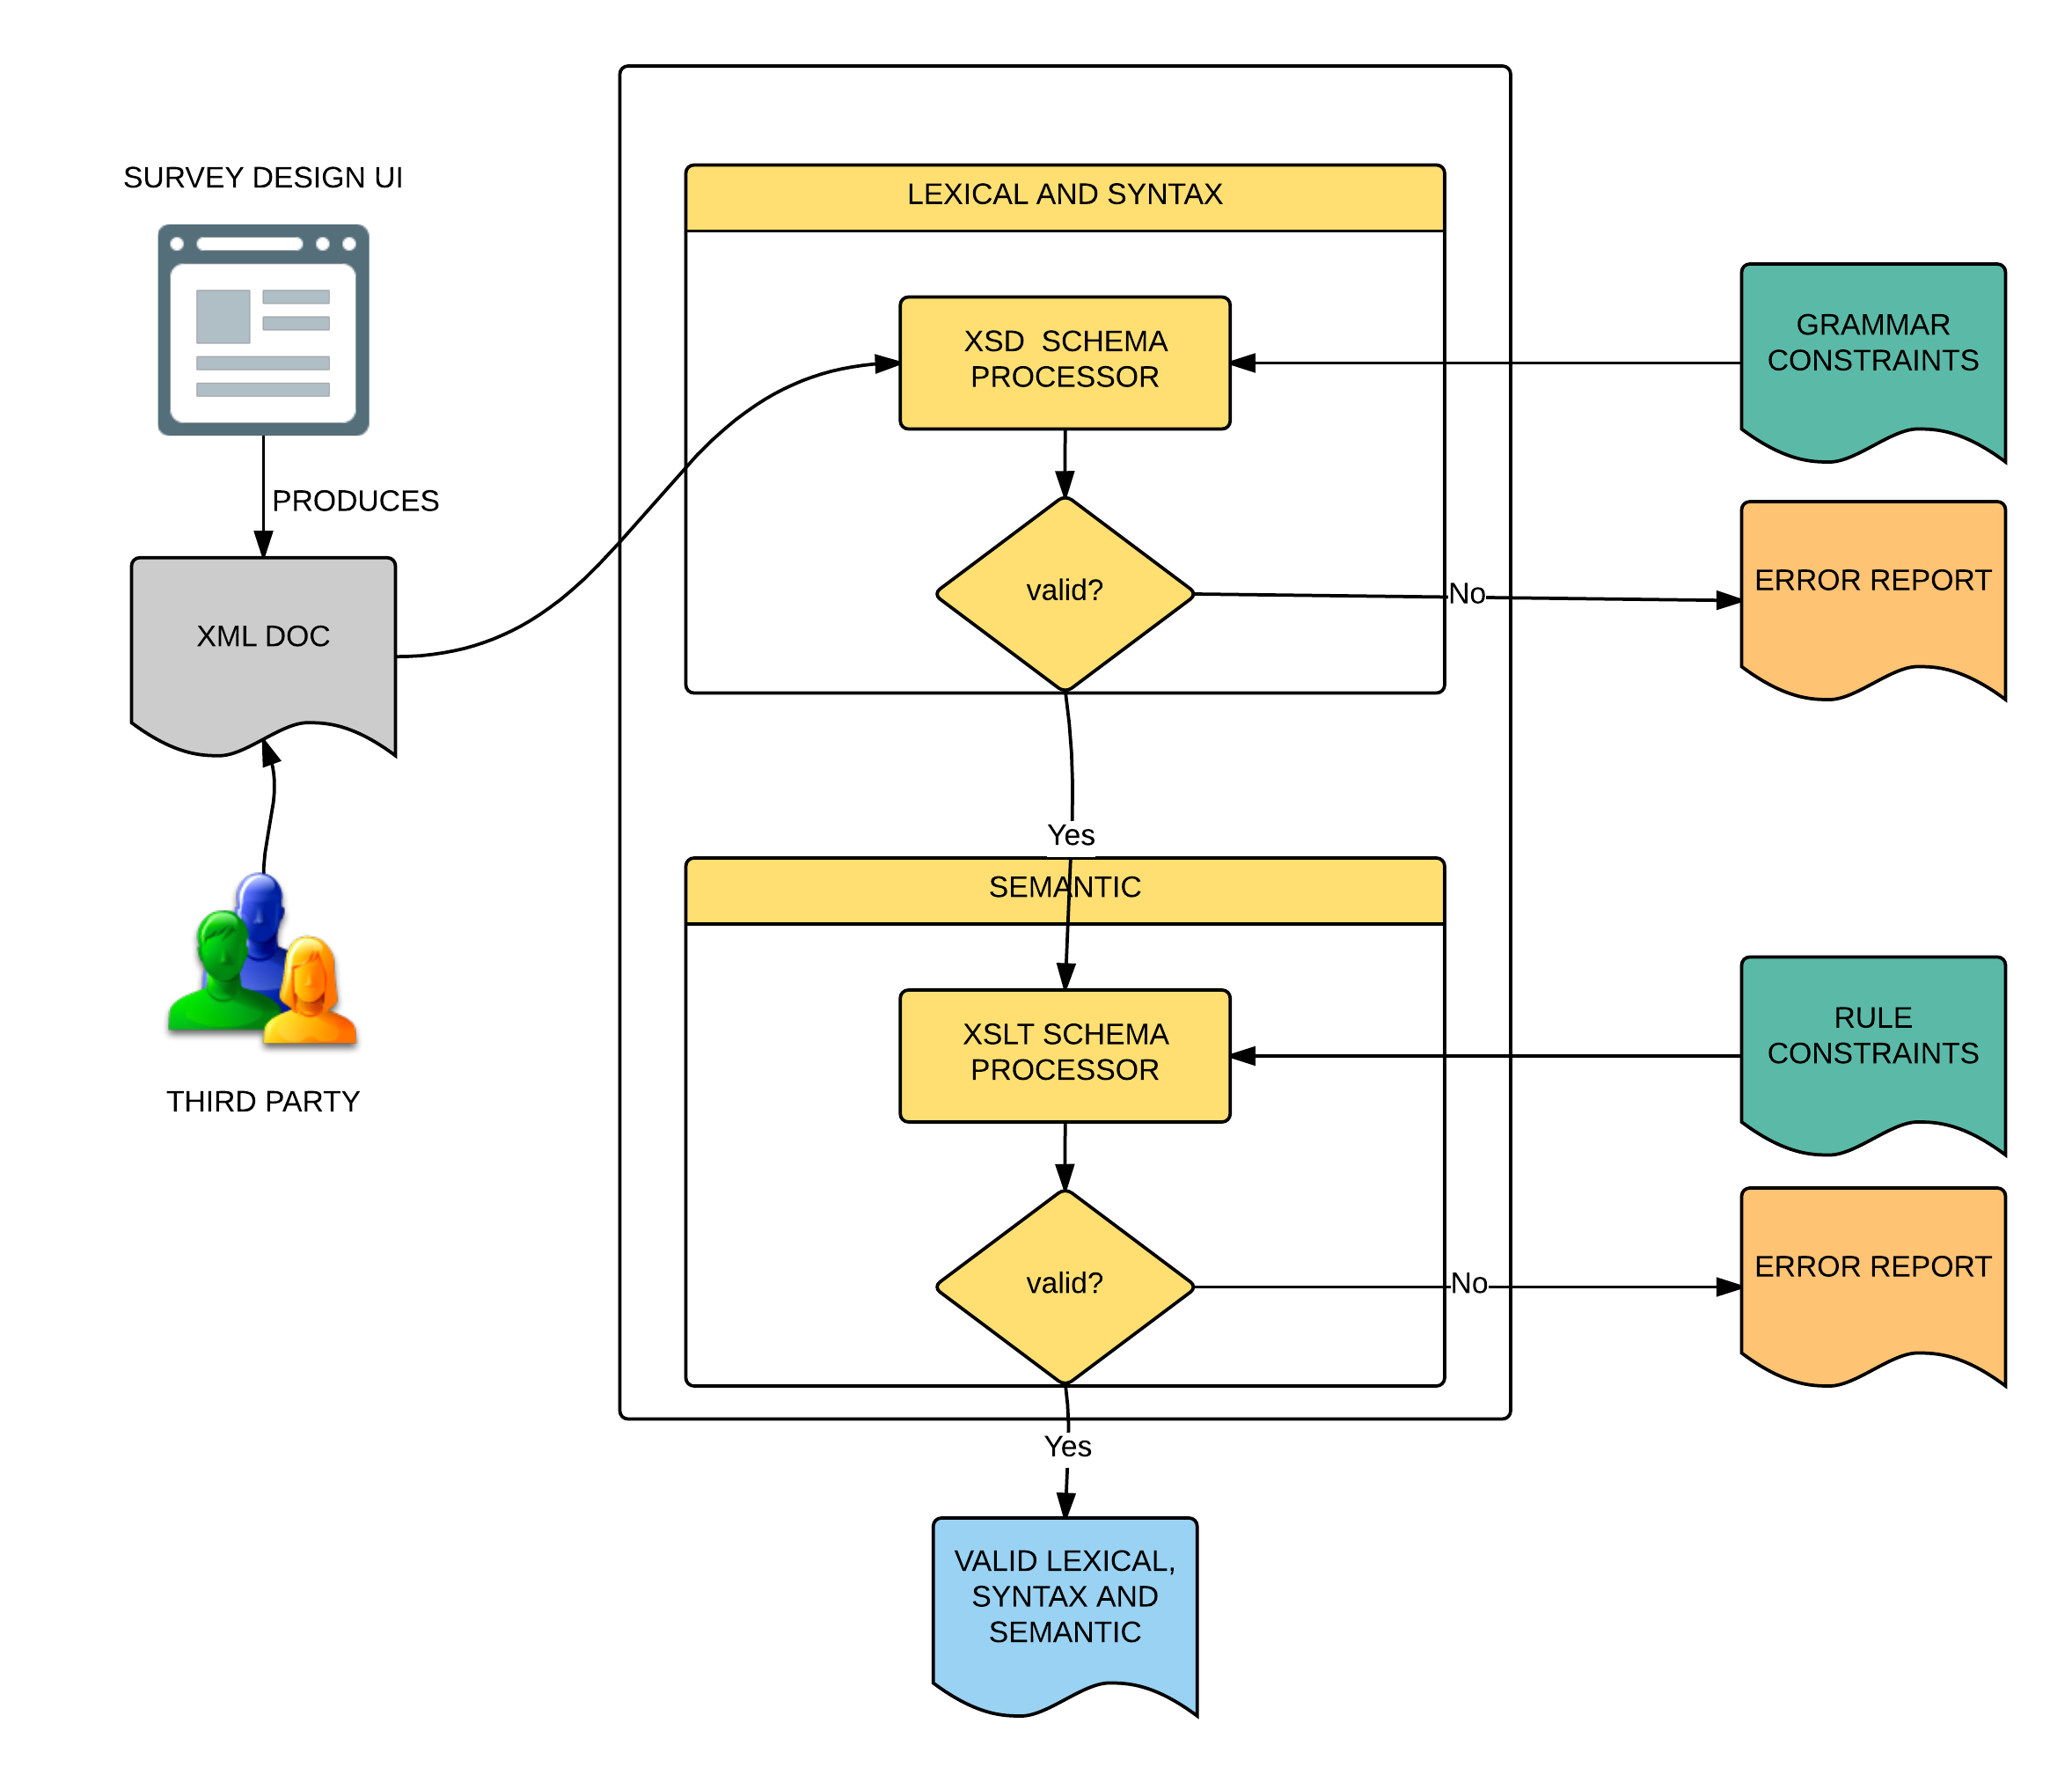
\includegraphics[max size={\textwidth}{\textheight}]{design/img/xmlValidation.png}
	\caption{Validation process of CAWIML}
	\label{fig:design:xmlValidation}
	\end{figure}

	An \gls{xml} document, that is presented either from our interface for designing questionnaires or from any third party, is passed to the validation component. In the first instance, the \gls{xml} schema processor takes our grammar constraints and an \gls{xml} document to verify whether the vocabulary, structures and data-types are valid. Two types of errors can arise from this operation, \emph{non-recoverable} errors that halt the process, i.e. the document is not well-formed (see Section \ref{sec:background:xml}) or \emph{recoverable} which are queued without interrupting the \gls{xml} processing.

	In the second instance, an \gls{xslt} processor takes our \gls{sch} rules, previously converted to the valid format accepted from this processor (see Section \ref{sec:background:sch}), and the \gls{xml} document to determine whether or not the relationships and domain specific rules are correct. The absence of any error at this stage confirms that the \gls{xml} document is valid according to our structure, data-types, integrity constraints and business rules and it is consequently ready to be parsed in our \gls{cawi} system for conducting the on-line survey.

	%We have found during the implementation that the reporting of errors is significantly less predictable for the the grammar-rules since \gls{xsd} schema only produces messages suited for debugging purposes \cite{masterthesis:madsen09}, being difficult to understand for people without any knowledge on schema languages. In contrast, \gls{sch} schema has permitted us to define customised messages that are more user-friendly and better suited for production environments.

	


